\section*{}
\begin{frame}{}
\begin{beamercolorbox}[colsep=1.5pt,rounded=true,shadow=true]{block body example}
    \huge{Chapter 4: Key Generation and Spatial Separation}
\end{beamercolorbox}
\vspace{2cm}
\textbf{Publication}:\\
C. Paschou, O. Johnson, Z. Zhu, and A. Doufexi.``Re-Defining Secure Distance for CSI-based Key Generation Protocols.'' In 2022 IEEE 95th Vehicular Technology Conference (VTC2022-Spring), pp. 1-6. IEEE, 2022.




\end{frame}


\section{Key Generation and Spatial Separation}
\begin{frame}{Motivation}
\begin{itemize}
\item \textbf{Common assumption in key generation:} In a rich scattering environment, when Eve is positioned half a wavelength $(0.5\lambda)$ apart, her channel is decorrelated to Bob's.
    \item This chapter points out that a distance of $0.5\lambda$ is not perfectly secure, even in idealistic environments with rich scattering.
    \item \textbf{Novel contribution:} If the distance of $0.5\lambda$ is not perfectly secure, then what is?
    \item Three geometric environments are studied:
    \begin{itemize}
        \item Isotropic scattering
        \item Omnidirectional scattering
        \item Restricted Uniform Angle-of-Arrival
    \end{itemize}
\end{itemize}
\end{frame}

\begin{frame}{Channel Correlation and Secrecy Degradation}
\framesubtitle{Worst case scenario}
\begin{figure}
    \centering
    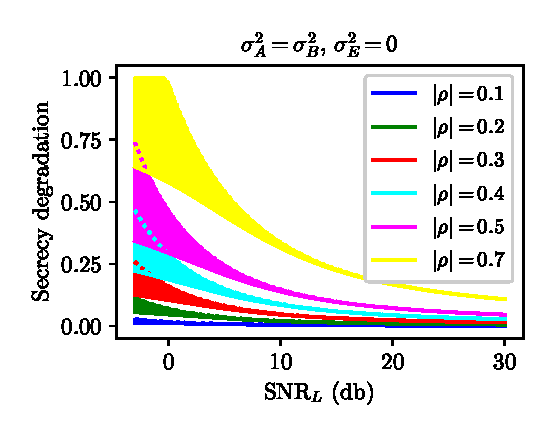
\includegraphics[scale = 0.9]{figures/key_generation_and_spatial_seperation/bounds_degrad.eps}
    \vspace{-0.5cm}
    \caption{Secrecy degradation as a function of $\rho$ and {SNR} at the legitimate users ($SNR_L = SNR_A = SNR_B$)}
\end{figure}
\end{frame}

\begin{frame}{Channel Correlation and Secrecy Degradation}
\framesubtitle{Equal SNR at all receivers}
\begin{figure}
    \centering
    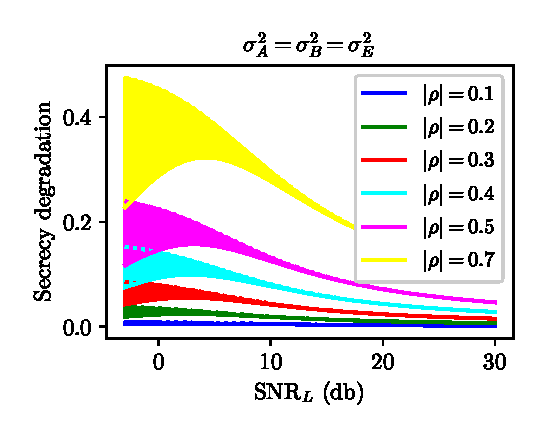
\includegraphics[scale = 0.9]{figures/key_generation_and_spatial_seperation/boundsDegrallequal.eps}
    \vspace{-0.5cm}
    \caption{Secrecy degradation as a function of $|\rho|$ and {SNR} at the legitimate users ($SNR_L = SNR_A = SNR_B$)}
\end{figure}
\end{frame}

\begin{frame}{Secure Distance}
\framesubtitle{Definition}    

\begin{definition}
    In a Cartesian coordinate system, let Eve be positioned at $E(x,y,z)$ and let $\rho(E(x,y,z))$ be the spatial channel correlation between Eve's channel and Bob's channel when Eve is positioned at $E(x,y,z)$. A distance $d_{s}$ is said to be $\epsilon$-secure if
    ~
    \begin{equation}
        |\rho(E(x,y,z))| < \epsilon \text{ for all } E(x,y,z)\notin S(B,d_s),
    \label{secure distance}\end{equation}
    where $S(B,d_{s})$ is the sphere with centre Bob's location and radius $d_{s}$. \label{dfn: secure distance}
\end{definition}
\end{frame}


\begin{frame}{Secure Distance}
\framesubtitle{Idealistic Scattering Environments}
\begin{figure}
    \centering
   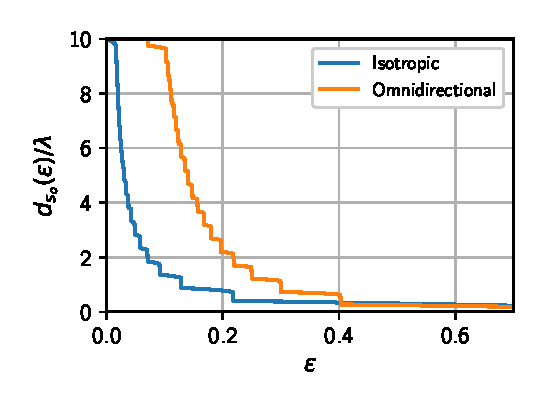
\includegraphics{figures/key_generation_and_spatial_seperation/securedistrichscattering.eps}
    \caption{The minimum secure distance for different thresholds.}
\end{figure} 
\end{frame}


%\begin{frame}{Secure Distance}
%\framesubtitle{Insights on the Derivation of Secure Distance}
%\begin{figure}
 %   \centering
  %  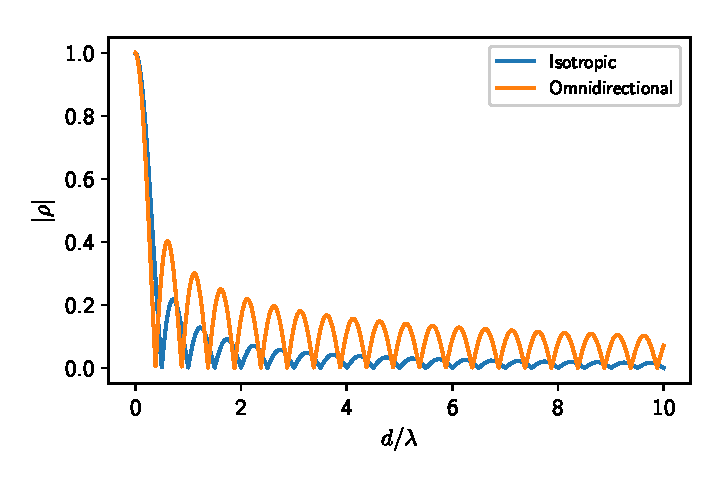
\includegraphics[scale = 0.78]{figures/key_generation_and_spatial_seperation/correlationRichscattering.eps}
   % \vspace{-0.5cm}
    %\caption{ The spatial channel correlation against the normalised distance between two
%receivers for the cases of isotropic diffuse field and omnidirectional diffuse field.}
%\end{figure}
%\end{frame}

\begin{frame}{Secure Distance}
\begin{example}
\textbf{Isotropic case:} The 0.1-secure distance is approximately 1.5$\lambda$.
\end{example}
\begin{example}
    \textbf{Omnidirectional case:} The 0.1-secure distance is approximately 10$\lambda$.
I.e., when Bob and Eve are equipped with dipole antennas, it takes approximately 10$\lambda$ for the channel correlation to drop below $0.1$.
\end{example}    
\end{frame}


\begin{frame}{Secure Distance}
\framesubtitle{Restricting the AoA}
\begin{figure}
    \centering
    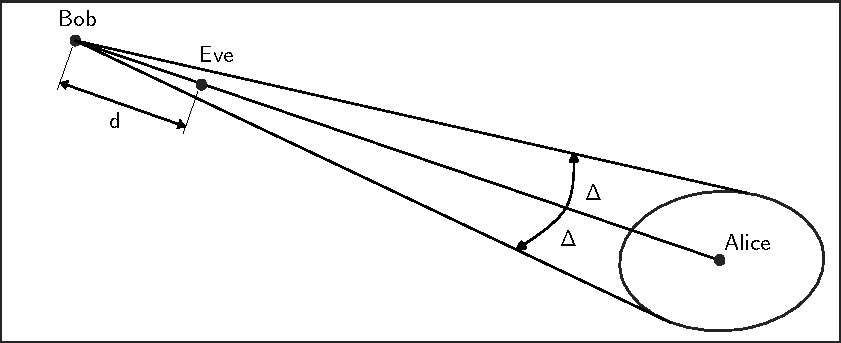
\includegraphics[scale = 0.7]{figures/key_generation_and_spatial_seperation/directional_optimal_eve.pdf}
    \caption{The restricted uniform AoA model. The spatial channel correlation maximises when Eve is inline with AB.}
    %\label{fig:enter-label}
\end{figure}    
\end{frame}

\begin{frame}{Secure Distance}
\framesubtitle{Restricting the Angle-of-Arrival}
\begin{figure}
    \centering
    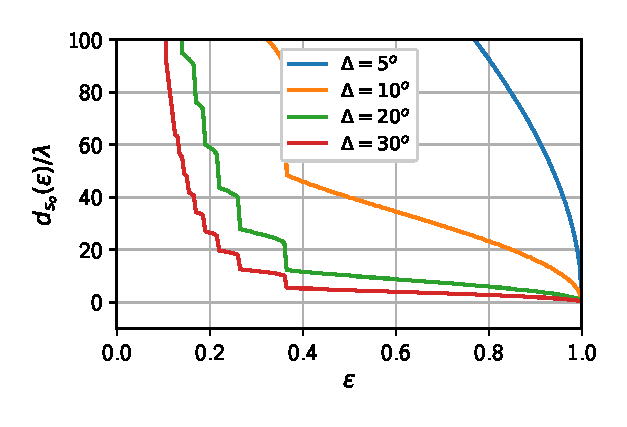
\includegraphics[scale = 0.9]{figures/key_generation_and_spatial_seperation/securedistDelta30zoom.eps}
    \caption{The minimum secure distance for different thresholds.}
   % \label{fig:enter-label}
\end{figure}
\end{frame}

\begin{frame}{Secure Distance}
\framesubtitle{Restricting the Angle-of-Arrival}
\begin{figure}
    \centering
    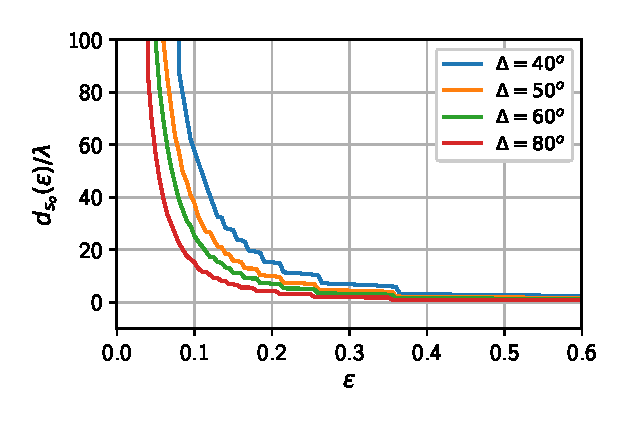
\includegraphics[scale = 0.9]{figures/key_generation_and_spatial_seperation/securedistDelta80zoom.eps}
    \caption{ Minimum secure distance such that the spatial correlation falls below $\epsilon$.}
\end{figure}
\end{frame}

\begin{frame}{Secure Distance}
\framesubtitle{Restring the Angle-of-Arrival}
\begin{figure}
    \centering
    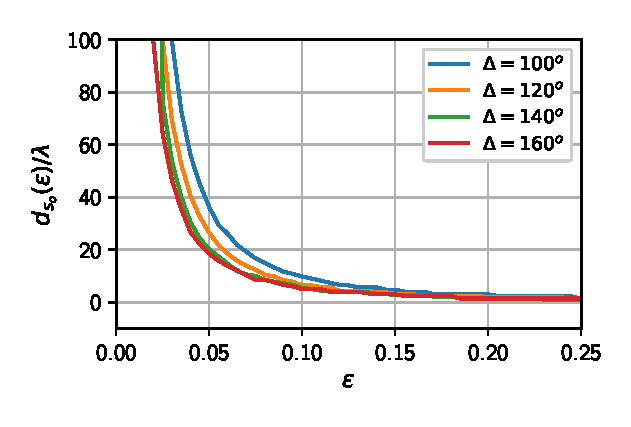
\includegraphics[scale = 0.9]{figures/key_generation_and_spatial_seperation/securedistDelta160zoom.eps}
    \caption{ Minimum secure distance such that the spatial correlation falls below $\epsilon$.}
    \label{fig:enter-label}
\end{figure}
\end{frame}

\begin{frame}{Secure Distance}
\framesubtitle{Restricting the Angle-of-Arrival}
 \begin{example}
Operating frequency: 2.4GHz
{AoA}-beamwidth: $80^0$ ($\Delta =40^o$). To achieve a maximal spatial correlation of 0.1, the eavesdropper needs to be distanced by at least 7m ($57\lambda$) from Bob. 
\end{example}

%\begin{example}
%Operating frequency: %$2.4GHz$
%{AoA}-beamwidth: $16^0$ ($\Delta =320^o$). To achieve a maximal spatial correlation of 0.1, the eavesdropper needs to be distanced by at least 2m ($19\lambda$) from Bob. 
%\end{example}
\begin{example}
For a minimum 0.1-secure distance of less than 1m, the beamwidth needs to be at least $200^o$ when the operating frequency is $f_c$=2.4GHz.
\end{example}
\end{frame}

\begin{frame}{Concluding Remarks}

\begin{itemize}
\item Even in an idealistic rich scattering, and assuming dipole antennas, the eavesdropper needs to be positioned at least ten wavelengths away to ensure negligible impact on secret key capacity;
\item In directive channels, the secure distance dramatically increases as the angle-of-arrival deviates from a uniform distribution across $(0, 2\pi]$;

\item \textbf{Suggestion:} For an effective and secure secrecy system, it is necessary to consider the influence of spatial channel correlation. Then restore the unpredictability of the key by eliminating the vulnerable key bits.

\end{itemize}   
\end{frame}